% !TEX root = ../YourName-Dissertation.tex

\chapter{Fast and Precise Side-channel Vulnerability Detection}\label{chapter3}
\section{Problem}
Side channels are ubiquitous in modern computer systems as sensitive information can leak through many mechanisms such as power consumption, execution time, electromagnetic radiation, and even sound~\cite{agrawal2002side,kar20178,chari1999towards,217605,genkin2014rsa}.  Among them, software side-channel attacks, such as cache attacks, memory page attacks, and controlled-channel attacks, are especially problematic as they do not require physical proximity~\cite{7163052,217543,217589,lee2017inferring,191010,liu2015last}. These attacks arise from shared micro-architectural components in a computer processor. By observing inadvertent interactions between two programs, attackers can infer program execution flows that manipulate secrets and guess secrets such as encryption keys~\cite{Osvik2006,Gullasch:2011:CGB:2006077.2006784,203878,10.1007/978-3-540-45238-6_6}.

The cause of most side-channel attacks is the combination of the hardware design and the vulnerable software. Existing countermeasures can be classified into two categories: fixing the software and adopting new hardware. Based on the discussion in \S\ref{chapter1} and \S\ref{chapter2}, fixing side-channel leakage sites in software is usually easier than adopting new hardware to defend against side-channel attacks. In order to eliminate these leakage sites, developers need to find potential leakage sites in a large code base. However, the manual process is tedious and error-prone. Recent work~\cite{203878} also suggests fixing old vulnerabilities can sometimes introduce new leakages.

Recent work has made good progress in detecting side-channel leakages automatically. Some tools (e.g., CacheD~\cite{203878}, CaSym~\cite{Brotzman19Casym}) have successfully identified unknown leakage sites in software products automatically. However, these tools have limitations.

First, although some tools~\cite{Brotzman19Casym} can find side-channel leakages in real-world software products, they can only analyze one code fragment at a time due to the expensive performance overhead. As a result, users of these tools sometimes need to cut off manually irrelevant code based on their experience. The trimming process is tedious and needs domain knowledge of the target software (e.g., which part of the code is more likely to have side-channel leakage sites). More importantly, if serious leakage sites are on the trimmed code, these tools will miss leakage sites as well.

Second, many tools perform the analysis at the level of intermediate representations (IR) instead of the machine code. It is a design decision to facilitate the implementations. While analyzing the IRs can simplify the implementation, it is not suitable for side-channel analysis.  Side-channel leakages are a low-level issue and only the low-level analysis can produce the most accurate results. For example, the IR-level branches are not necessarily a superset or a subset of machine-code level branches. Besides, compiler optimizations can eliminate the IR-level branches with conditional moves, and the converse could also happen. Moreover, translating the machine code into IRs can cause a significant overhead for the trace analysis, as we will discuss in the dissertation.

To overcome the above problems, we propose a fast and precise method to detect the side-channel leakages in real-world software products. We examine the bottleneck of current symbolic execution approaches and optimize it to work on real-world cryptography systems. Unlike previous methods, our tool analyzes the machine instructions, which can give more precision than traditional IR-based approaches. We evaluate our tool on popular cryptography libraries including OpenSSL, mbedTLS, Libgcrypt, and Monocypher. The evaluation results show that our tool can identify previous side-channel leakages as well as find new leakages. Compared with recent tools~\cite{203878,217537,Wichelmann:2018:MFF:3274694.3274741}, our tool is 3--100x faster while finding all the leakages when we evaluate on the same benchmarks. In addition, our tool finds new side-channel vulnerabilities missed by the previous work. 

\section{Background and Threat Model}
\subsection{Micro-architectures}
Many side-channel attacks are architecture-dependent. To facilitate the illustration, we present some necessary backgrounds in this section.

During the evolution of the computer architecture, researchers found that CPUs process data much faster than the main memory (DRAM) can supply. As a result, CPUs adopted a hierarchy memory architecture to bridge the performance gap between the CPUs and the main memory. By storing extra copies of recently accessed data and code in a smaller but faster memory, the software can get its most recently accessed code and data in a shorter time.

Figure~\ref{fig:memory_hierarchy} shows the overview of one example of the hierarchy memory architecture. For a CPU with multiple cores, each core has two private level-1 (L1) cache, an instruction cache (iCache), and a data cache (dCache). Because instructions and data have different access patterns, separating iCache and dCache makes it possible for CPUs to fetch the code and data simultaneously and improve performance. Followed by the level-1 cache, each core also has the unified, private level-2 cache for both the code and the data. The level-3 cache is the last level cache (LLC). The LLC is shared among all the cores.
The main memory is at the bottom of the memory hierarchy.
\begin{figure}[ht]
  \centering
  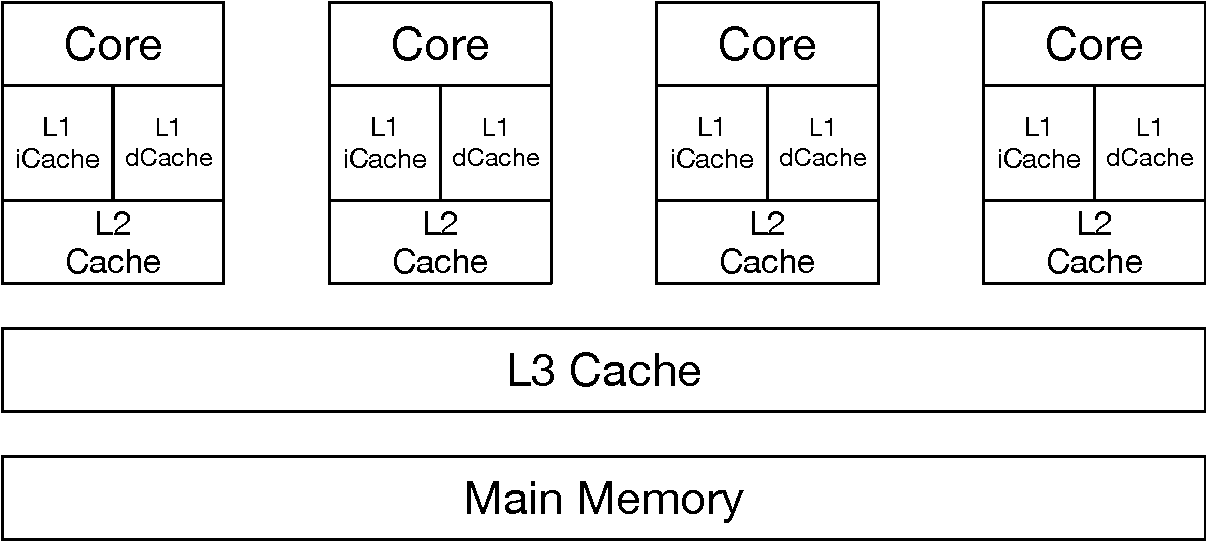
\includegraphics[width=.65\columnwidth]{./figures/chapter3/architecture.pdf}
  \caption{Computer memory hierarchy. The hierarchy is designed to minimise the access time with the relatively low cost. It is the root cause of many side-channel attacks.}\label{fig:memory_hierarchy}
\end{figure}

The current computer memory hierarchy opens the way for side-channel attacks from two aspects. First, the architecture relies on the system software to manage the memory, which becomes a problem in a threat model when the operating system is not untrusted (e.g., Intel SGX). Second, the size of the cache is smaller than the main memory. It is possible that different units in the main memory share the same address in the cache.
\begin{figure}[ht]
  \centering
  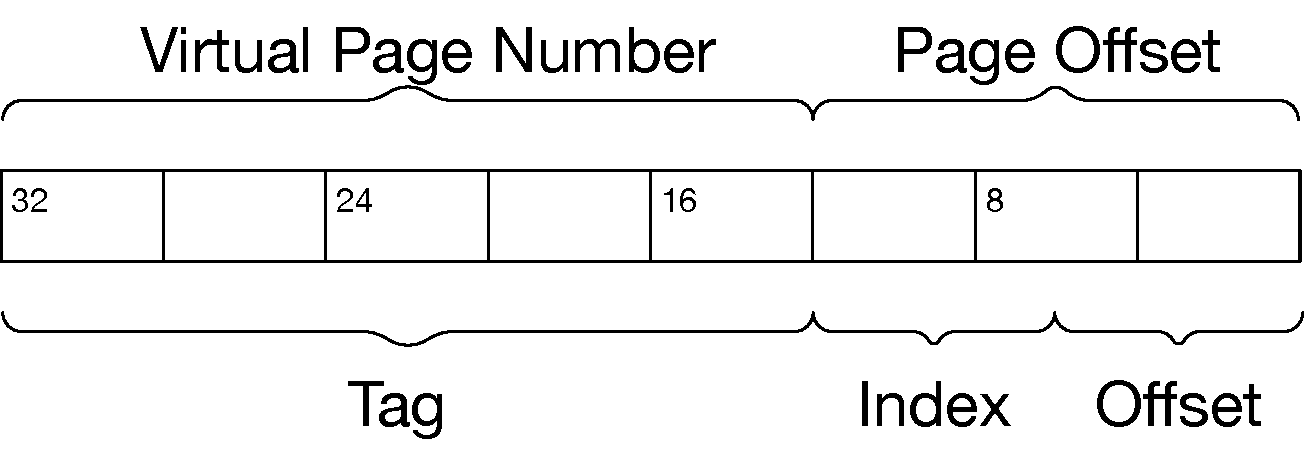
\includegraphics[width=.65\columnwidth]{./figures/chapter3/address.pdf}
  \caption{Memory addressing}\label{fig:memory_address}
\end{figure}

In modern CPUs, L1 and L2 caches are traditional N-way set associate caches. That is, the cache is divided into several cache sets, and each set contains several cache lines. The cache line is the atomic unit. As shown in Figure~\ref{fig:memory_address}, we can determine whether the data is in the cache with the following steps.  Given an address, the CPU uses the \textsf{Index} field of the address to locate the cache set that the address should reside in. After that, it tries to use the \textsf{Tag} field to match every cache line inside the set line. If the CPU can locate a cache line with the same tag and the valid bit is set, then a cache hit occurs. The CPUs use a similar process to manage the main memory. The main memory is divided into many units called pages. As shown in Figure~\ref{fig:memory_address},
the translation process keeps the bottom bits same while using the top bits to map the Physical Page Numbers to Virtual Page Numbers. 

\subsection{Threat Model}
We assume that an attacker shares the same hardware platform with the victim.
The attacker attempts to retrieve sensitive information through address-based side-channel attacks. The attacker has no direct access to the victim's data, but he can probe the memory or cache at each program point. Here are a few examples.
\begin{enumerate}
  \item A host machine has several virtual machines (VMs). The victim runs the application inside one VM. An attacker can control one VM and probe the process running on the other VM.
  \item  In a shielding system~\cite{arnautov2016scone,schuster2015vc3}, a malicious operating system can extract sensitive information from protected user-level applications.
  \item A ring-3 application can probe some sensitive information inside the kernel.
\end{enumerate}

In reality, attackers may face many possible obstacles, such as the noisy observations of the memory or cache. However, in this research, we assume the attacker has noise-free observations as in previous work~\cite{203878,182946,Brotzman19Casym}. The threat model captures most address-based side-channel attacks and apply to the three attack models: 1) time-based attacks, 2) access-based attacks, 3) trace-based attacks. We only consider deterministic programs and assume an attacker has access to the source code or binary executable of the target program.

\section{Limitations of Previous Side-channel Leakage Detection Tools}
In this section, we introduce two limitations of current side-channel leakage detection tools. The first is that some tools have some false positives or false negatives. The second is that current tools are not fast enough to analyze side-channel leakages in real-world software.


\subsection{Imprecision}
In this dissertation, we study two types of side-channel leakage code patterns. The intuition is that the target application shows different control flows or data flows when it processes different sensitive input data. We refer them as \textit{secret-dependent control flow transfers} and \textit{secret-dependent data accesses}. Unlike previous work, our tool works on the machine code, which is more precise than previous tools that work on the source code or the intermediate representation.
\subsubsection{Control Flow}
\begin{figure}[ht]
  \begin{minipage}{0.45\linewidth}
    \begin{lstlisting}[xleftmargin=.05\textwidth, xrightmargin=.0\textwidth, frame=none]
int example1(uint8_t k, uint32_t m) { 
  uint32_t b = (k & m) >> 7; // m = 0
  if (b) {
    ...    // Branch 1
  } else {
    ...    // Branch 2
  }
  ...
}
\end{lstlisting}
  \end{minipage}
  \hfill
  \begin{minipage}{0.45\linewidth}
    \begin{lstlisting}[xleftmargin=.05\textwidth, xrightmargin=.00\textwidth, frame=none, numbers=none, mathescape=true]
push  ebp
mov   ebp, esp
movzx eax, [addr_k]    
and   eax, [addr_me] 
shr   eax, 0x7           
test  eax, eax
jne   branch 2
...
\end{lstlisting}
  \end{minipage}\caption*{(a) A False Negative}

  \begin{minipage}{0.45\linewidth}
    \begin{lstlisting}[xleftmargin=.05\textwidth, xrightmargin=.0\textwidth, frame=none]
int example2(uint16_t k) {
  int res;
  if (k > 8) {
    res = 0;
  } else {
    res = 1;
  }
  return res;
}
\end{lstlisting}
  \end{minipage}
  \hfill
  \begin{minipage}{0.45\linewidth}
    \begin{lstlisting}[xleftmargin=.05\textwidth, xrightmargin=.00\textwidth, frame=none, numbers=none, mathescape=true]
xor   eax, eax
cmp   [addr_k], 8
setbe al
xor   edx, edx
ret
\end{lstlisting}
  \end{minipage}\caption*{(b) A False Positive}
  \caption{Secret-dependent control-flow transfers}\label{fig:chapter3:cf}
\end{figure}

If the input-sensitive data can affect the victim program's control flow, then an attacker can infer the sensitive data by observing the control flow during the execution. Figure~\ref{fig:chapter3:cf}(a) shows such an example. The function takes a public value \textsf{m} and a secret \textsf{k} as the inputs. The code at line 2 ensures that the lower 7 bits of the value \textsf{k} do not affect the value \textsf{b}. However, depending on the value of \text{m}, the code snippet in Figure~\ref{fig:chapter3:cf}(a) may have a leakage site. If the eighth bit of \textsf{m} is 1, then an attacker can infer the eighth bit of \textsf{k} by observing the branch at line 4 or line 6. The right figure shows the corresponding machine code. It has a conditional jump instruction \textsf{jne}. The sensitive input \textsf{k} can affect the program counter (the rip register), which is the root cause of the side-channel leakages.

However, the if-else branch does not always indicate there is a potential leakage site. Figure~\ref{fig:chapter3:cf}(b) shows a different situation. While the sensitive input \textsf{k} can affect the if-else branch, the compiler removes the branch with a conditional set instruction.  The opposite situation is the same. For example, recent work tries to use bit masking to rewrite the program with control flows. However, for some situations~\cite{Coppens:2009:PMT:1607723.1608124}, compilers (e.g., GCC) optimize the code too much (from a security view) and remove the unnecessary copy by reintroducing conditional moves.
\subsubsection{Data Flow}
\begin{figure}[ht]
  \begin{minipage}{0.4\linewidth}
    \begin{lstlisting}[xleftmargin=.15\textwidth, xrightmargin=.0\textwidth, frame=none]
uint8_t T[128];
...
int example3(uint8_t k, uint32_t m){
  uint32_t index = m;
  index = index + k % 128;
  uint8_t t = T[index];
  ...
}
\end{lstlisting}
  \end{minipage}
  \hfill
  \begin{minipage}{0.4\linewidth}
    \begin{lstlisting}[xleftmargin=.15\textwidth, xrightmargin=.00\textwidth, frame=none, numbers=none, mathescape=true]
...
lea    edx, [addr_T]
mov    eax, [addr_k]
and    eax, 0x7f
add    eax, [addr_m]
movzx  eax, [addr_T + eax*1]
...
\end{lstlisting}
  \end{minipage}\caption*{(a) A True Leakage}

  \begin{minipage}{0.4\linewidth}
    \begin{lstlisting}[xleftmargin=.15\textwidth, xrightmargin=.0\textwidth, frame=none]
uint8_t T[32];
...
int example4(uint8_t k, uint32_t m){
  uint32_t index = m;
  index = index + k % 32;
  uint8_t t = T[index];
  ...
}
\end{lstlisting}
  \end{minipage}
  \hfill
  \begin{minipage}{0.4\linewidth}
    \begin{lstlisting}[xleftmargin=.15\textwidth, xrightmargin=.00\textwidth, frame=none, numbers=none, mathescape=true]
...
lea    edx, [addr_T]
mov    eax, [addr_k]
and    eax, 0x3f
add    eax, [addr_m]
movzx  eax, [addr_T + eax*1]
...
\end{lstlisting}
  \end{minipage}\caption*{(b) A False Positive}
  \caption{Secret-dependent data accesses}\label{fig:chapter3:da}
\end{figure}

Figure~\ref{fig:chapter3:da} shows an example of secret-dependent data access. \textsf{T} is an array with 128 elements. The size of each element is one byte. So the total size of the array is 128 bytes. Suppose an attacker can observe the memory access at the granularity of one cache lines (64 Bytes), then it is not possible to hold all the data inside the one cache line. An attacker can get some information of the value \textsf{secret} in Figure~\ref{fig:chapter3:da}(a) by observing the cache line access. Figure~\ref{fig:chapter3:da}(b) shows a different example. In this example, only 32 different elements can be accessed in the array and the size of the array is 32 bytes, which is smaller than the size of a cache line. Depending on the base address of the array, the array can be stored in one cache line or two consecutive cache lines. Therefore, such a code may still be vulnerable to side-channel vulnerabilities. However, existing tools (e.g., CacheD~\cite{203878}) use a concrete base address. Under the circumstance, these tools may miss such vulnerabilities.

\subsection{Performance}
The second limitation of current side-channel detection tools is the performance bottleneck, especially for tools based on symbolic analysis. For example, CaSym~\cite{Brotzman19Casym} can only analyze small programs. CacheD performs better than CaSym. However, it still cannot handle large programs such as RSA directly. It uses some domain knowledge to analyze only part of the program. The expensive cost comes from the symbolic execution. Symbolic execution can be used to explore all the possible paths, which is useful for many tasks.
Nevertheless, it is significantly less likely for cache side-channel bugs in crypto primitives. Cryptography primitives are more likely to have an even coverage of different paths (based on pseudo-random cipher states), and a branch-based side-channel is vulnerable from the very first branch on secret data, making complex path conditions less often relevant. Therefore, we choose to analyze a trace instead of the whole path. Another bottleneck is that the IR. While the IR can significantly decrease the difficulty of the implementation, it also gives introduce an average of 10x of the overall overhead. Third, using SMT solving can be convenient because of its generality, and it is commonly used for its precision when checking branch feasibility in symbolic execution. But the decision problems that an SMT solver handles are typically at least NP-hard. On the other hand, we can use some methods to avoid the expensive SMT solving and find side-channel leakages more efficiently.

\section{Method}\label{chapter3:method}
\begin{figure}[ht]
  \centering
  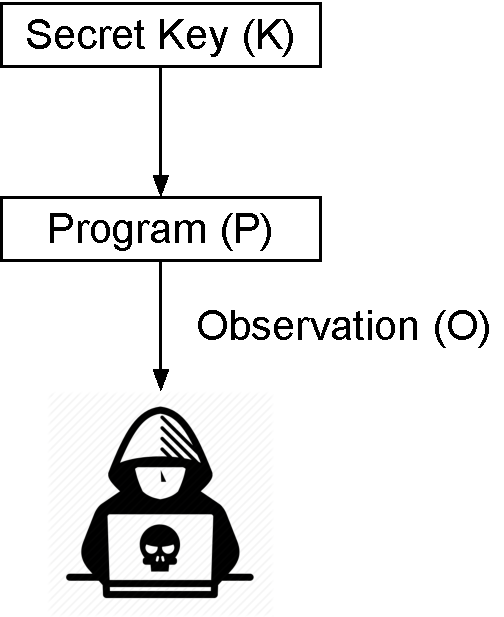
\includegraphics[width=.3\columnwidth]{./figures/chapter3/attack.pdf}
  \caption{A side-channel attack}\label{fig:side-channel-attack}
\end{figure}

In this section, we give necessary definitions and notations for dealing with
programs and side-channels.

Shown in Figure~\ref{fig:side-channel-attack}, a side-channel attack can be formulated into the following steps.  A program ($\beta$) has $K$ as its sensitive input (e.g., the encryption key) and $M$ as its the public input (e.g., the plaintext). In a real execution, an adversary may have
some observations ($O$) of the program. Examples of these observations include the timing, CPU usages, and electromagnetic signals (EM). In this dissertation, we use secret-dependent control flows and secret-dependent data
accesses as observations.

With the above definition, we have the following mapping between $\beta$, $K$, $M$, and $O$:
\begin{displaymath}
  \beta(K, M) \rightarrow O
\end{displaymath}


We model a side-channel in the following way. An adversary does not have
access to $K$, but he knows $\beta$, $M$, and $O$. For one execution of a
deterministic program, once $k \in K$ and $m \in M$ are fixed, the observation
($o \in O$) should also be determined. An attacker knows $\beta$, $o$,
and $m$. The attacker wants to infer the value of $k$. Moreover, we assume
an attacker can change the public input ($m \in M$) while keeping the secret input $k$. The threat model is similar to a chosen-plaintext attack.
We now discuss how to model observations ($O$),
which are the direct information that an adversary gets during the attack.

For one execution, a program ($\beta$) has many temporary values ($t_i \in
  T$). Once $\beta$ (program), $k$ (secret), and $m$ (message, public) are
determined, $t_i$ is also fixed. Therefore, $ t_i = f_i(\beta, k, m)$, where $f_
  i$ is a function that maps between $t_i$ and ($\beta$, $k$, $m$). In the chapter,
we consider two code patterns that can be exploited by an attacker,
\emph{secret-dependent control transfers} and \emph{secret-dependent data
  accesses}. 

\subsection{Secret-dependent Control Transfers}
A control-flow path is secret-dependent if different input-sensitive keys
($K$) can lead to different branch conditions.
We define a branch to be secret-dependent if
$$\exists k_{i1}, k_{i2} \in K, m \in M, \,f_i(\beta, k_{i1}, m) \neq f_i(\beta, k_{i2}, m) \land PC,$$

\noindent where $PC$ represents the path condition. An adversary can observe which branch the code executes if the branch condition
equals $t_b$. We use the constraint $c_i : f_i(\beta, k, m) = t_b$ to model
the observation ($o$) on secret-dependent control-transfers. Note that in the
above definition, $m$ is also a variable. So it is possible for some $m \in M$,
we cannot find a pair of two different $k_{i1}$ and $k_{i2}$ to satisfy the above inequation. For example, in Figure~\ref{fig:chapter3:cf}, if $m = \mathtt{0}$, the function \textsf{example1} will always execute the branch 2. However, if $m = \mathtt{0xffffffff}$ and $k = \mathtt{0}$, the function \textsf{example1} executes the branch 1 and the function \textsf{example1} executes the branch 2 when $k = \mathtt{0xf000000}$.


\subsection{Secret-dependent Data Accesses}
Similar to secret-dependent control-flow transfers, a data access operation is
secret-dependent if different input sensitive keys ($K$) cause access to different memory addresses. We use the model from CacheD~\cite{203878}. The low $L$ bits of the address are generally unimportant in side-channels.

A data access is secret-dependent if

$$\exists k_{i1}, k_{i2} \in K, m \in M,\,f_i(\beta, k_{i1}, m) >> L \neq f_i(\beta, k_{i2}, m) >> L \land PC.$$

If the memory access equals to $t_b$, we can use the constraint $c_i :
  f_i(\beta, k, m) >> L = t_b >> L$ to model the observation on secret-dependent
data accesses. Let us take a look at the examples in Figure~\ref{fig:chapter3:da}(a).
Suppose the base address of the array \textsf{T} is 10. We symbolize both the $k$ and $m$. The formula that represents the memory access at line 6 is $10 + m + (k \mod 128)$. Therefore, we have the formula $(10 + m + (k_1 \mod 128)) >> 6  \neq (10 + m + (k_2 \mod 128)) >> 6$.
Here is one possible solution: $m = 0, k_1 = 0, k_2 = 127$. In fact, for any $m$, we can always find possible $k_1$ and $k_2$ that satisfy the above inequation. It is a true leakage. The leakage can also be identified by previous tools such as CacheD. Similarly, we can model the memory access at line 6 with the formula:  $10 + m + (k_1 \mod 32) >> 6  \neq 10 + m + (k_2 \mod 32) >> 6$. If $m = 0$, we cannot find satisfiable $k_1$ and $k_2$ for the above inequation, which indicates that it will always access the same cache line at line 6. However, it is possible that for some $m \in M$, we can find such a pair of $k_1$ and $k_2$ ($m = 53, k_1 = 1, k_2 = 0$). If the actual public input is $0$, existing tools (e.g., CacheD) can miss such a vulnerability. On the other hand, our tool can identify the leakages precisely.

\section{Scalability}
\subsection{Trace-oriented Symbolic Execution}
Symbolic execution is notorious for its expensive performance cost.
Previous trace-oriented symbolic execution
work~\cite{203878,Chattopadhyay:2017:QIL:3127041.3127044} has serious
performance bottlenecks. As a result, these approaches either apply only to
small programs~\cite{Chattopadhyay:2017:QIL:3127041.3127044} or require
domain knowledge~\cite{Wang:2007:NCD:1250662.1250723} to simplify the analysis.
These tools interpret each
instruction and update memory cells and registers with formulas that
captured the semantics of the execution and search different input values that
can lead to different execution behaviors using a constraint solver.
We implement the approach presented in \S\ref{chapter3:method} and model the side-channels as formulas. While the tools can analyze some simple cases such as AES, it cannot handle complicated examples such as RSA.
We observe that finding side-channels using symbolic execution differs from
traditional symbolic execution, and the symbolic analysis approach can be optimized to be as efficient
as other methods.

\subsection{Interpret Instructions Symbolically}
Existing binary analysis frameworks~\cite{shoshitaishvili2016state,
  10.1007/978-3-642-22110-1_37, song2008bitblaze} translate machine instructions into
intermediate languages (IR) to simplify analysis since
the variety of machine instructions is
enormous, and their semantics is complex. The Intel Developer
Manual~\cite{intelsys} documents more than 1000 different x86 instructions.
Unfortunately, the IR layer, which
reduces the workload of these tools, is not suitable for side-channels
analysis because
IR-based or source code side-channels analyses do not represent the executed instructions accurate enough to analyze fully their control and memory accesses.
For example, a compiler may use conditional moves or bitwise operations to eliminate
branches. Also, as some IRs are not a superset or a subset of ISA,
it is hard to rule out conditional jumps introduced by IR and add real branches
eliminated by IR transformations.

Moreover, the IR causes significant overhead~\cite{217563}.
Translating machine instructions into IR is time-consuming. For example,
REIL IR~\cite{dullien2009reil}, adopted in CacheS~\cite{236338}, has multiple
transform processes, from binary to VEX IR, BAP IR, and finally REIL IR\@.
Also, IR increases the total number of instructions. For example, x86
instruction \textit{test eax, eax} transfers into 18 REIL IR instructions.

\textbf{Our Solution}
We abandoned IR and expended the effort to implement
symbolic execution directly on x86 instructions.
Table~\ref{scala:ir} shows that eliminating the IR reduces the number
of instructions examined during analysis. Previous works~\cite{217563} also
adopted a similar approach to speed up fuzzing. Our implementation differs
from that work in two aspects: 1) We use complete constraints. 2) We run the
symbolic execution on one execution path each time. Our approach is approximately 30 times faster than using an IR (transferring ISA into IR and
symbolically executing it).

\begin{table}[ht]
  \centering\small\footnotesize
  \caption{The number of x86,  % instructions and the number of 
    REIL IR, and VEX IR instructions on the traces of crypto programs.}
  \label{scala:ir}
  \resizebox{.8\columnwidth}{!}{%

    \begin{tabular}{cccc}
      \hline
                        & \begin{tabular}[c]{@{}c@{}}Number of\\ x86 Instructions\end{tabular} & \begin{tabular}[c]{@{}c@{}}Number of\\ VEX IR\end{tabular} & \begin{tabular}[c]{@{}c@{}}Number of\\ REIL IR\end{tabular} \\ \hline
      AES OpenSSL 0.9.7 & $1,704$                    & $23,938$ (15x)             & $62,045$ (36x)             \\
      DES OpenSSL 0.9.7 & $2,976$                    & $41,897$ (15x)             & $100,365$ (33x)            \\
      RSA OpenSSL 0.9.7 & $1.6*10^7$                 & $2.4*10^8$ (15x)           & $5.9*10^8$ (37x)           \\
      RSA mbedTLS 2.5   & $2.2*10^7$                 & $3.1*10^8$ (15x)           & $8.6*10^8$  (39x)          \\ \hline
    \end{tabular}
  }
\end{table}

\subsection{Constraint Solving}
As discussed in the previous section, the problem of identifying
side-channels can be reduced to the question below.

\begin{quote}
  \textit{Can we find two different input variables $k_1, k_2 \in K$ that
    satisfy the formula $f_a(k_1) \neq f_a(k_2)$?}
\end{quote}

Existing approaches rely on satisfiability modulo theories (SMT) solvers
(e.g., Z3~\cite{DeMoura:2008:ZES:1792734.1792766}) to find satisfying assignments to
$k_1$ and $k_2$.
While this is a universal approach to solving constraints,
for constraints of this form, using custom
heuristics and testing is much more efficient in practice. Constraint
solving is a decision problem expressed in logic formulas. SMT solvers
transfer the SMT formula into the boolean conjunctive normal
form (CNF) and feed it into the internal boolean satisfiability
problem (SAT) solver. The translation process, called ``bit blasting'',
is time-consuming. Also, as the SAT problem is a well-known NP-complete
problem, it is hard to deal for huge formulas. Despite the rapid improvement
in SMT solvers in recent years, constraint solving remains one of
the obstacles to scaling the analysis of real-world crypto-systems.

\textbf{Our Solution}
Instead of feeding the formula $f_a(k_1) \neq f_a(k_2)$ into a SMT solver, we
randomly pick $k_1, k_2 \in K$ and test them if they satisfy the
formula. Our solution is based on the following intuition. For most combination
of $(k_{1}, k_{2} )$, $f_a(k_1) \neq f_a(k_2)$. As long as
$f_a$ is not a constant function, such $k_1, k_2$ must exist. For example,
suppose each time we only have 5\% chance to find such $k_1, k_2$, then after we
test with different input combination with 100 times, we have $1 -
  (1-0.05)^{100} = 99.6\%$ chance find such $k_1, k_2$. This type of random algorithm works well for our problem.

\section{Design and Implementation}
\subsection{Trace Logging}
The trace information can be logged via some emulators (e.g., QEMU~\cite{bellard2005qemu}) or dynamic binary instrumentation tools (DBI).
In this work, we run a program with the concrete input under the DBI to record execution traces.
The trace data has the following information:
\begin{itemize}
  \item Each instruction mnemonics and its memory address.
  \item The operands of each instruction and their concrete values during the runtime.
  \item The value of EFLAGS registers.
  \item The memory address and the length of the sensitive information.
        Most crypto libraries store sensitive information in arrays,
        variables or contiguous buffer.
\end{itemize}

\subsection{Instruction Level Symbolic Execution}
\label{InstructionSE}
The primary purpose of the step is to generate constraints of the input sensitive information from the execution trace. If we give the target program a new input which is different from the original input that was used to generate the execution trace but still satisfies these constraints, an attacker will have the same observations on control-flow transfers and data-access patterns.

The tool runs symbolic execution on top of execution traces. At the beginning of the symbolic execution, the tool creates new symbols for each byte in the raw buffer. For other data in the register or memory at the beginning, we use actual values from the runtime execution information. During the symbolic execution for each instruction, the tool updates every variable in the memory and registers with a math formula. The formula is made up of concrete values and symbols accumulated through the symbolic execution. We implement several rules to simplify the formulas. For each formula, the tool will check whether it can be reduced into a concrete values (e.g., $k_1+12-k_1 = 12$ ). If so, the tool will only use the concrete values in the following symbolic execution.

\subsubsection{Verification and Optimization}
We run the symbolic execution (SE) on the x86 instructions. In other words, we do not rely on any intermediate languages to simplify the implementation of symbolic execution. While the implementation itself has a lot of benefits (better performance, accurate memory model), we need to implement the symbolic execution rules for each x86 instruction.
However, due to the complexity of x86, mistakes inevitable. Therefore, we verify the correctness of the SE engine during the execution.
The tool will collect the runtime execution information (register values, memory values) and compare them with the formula generated from the symbolic execution. Whenever the tool finishes the symbolic execution of each instruction, the tool will compare the formula for each symbol and its actual value. If the two values do not match, we check the code and fix the error. Also, if the formula does not contain any symbols, the tool will use the concrete value instead of symbolic execution.

\subsubsection{Secret-dependent Control-flows}
An adversary can infer sensitive information from secret dependent control-flows. There are two kinds of control-transfer instructions: the unconditional control-transfer instructions and the conditional transfer instructions.
The unconditional instructions, such as CALL, JUMP, and RET, transfer control flows from one code segment location to another. Since the transfer is independent of the input sensitive information, an attacker is not able to infer any sensitive information from the control-flow.
So unconditional control-transfer does not leak any information based on our threat model. During the symbolic execution, we update the register information and memory cells with new formulas accordingly.

The conditional control-flow transfer instructions, such as conditional jumps, depending on CPU states, may or may not transfer control flows. For conditional jumps, the CPU will test if certain condition flag
(e.g., CF = 0, ZF =1) is met and jump to certain branches, respectively.
The symbolic engine will compute the flag and represent the flag in a symbol
formula. Because we are running on a symbolic execution on an execution trace, we know which branch is executed.
If a conditional jump uses the CPU status flag, we will generate the constraint accordingly.

For examples, considering the following x86 code snippet.

\begin{lstlisting}[xleftmargin=.2\textwidth, xrightmargin=.2\textwidth, frame=none,numbers=none][h]
...
0x0000e781      add dword [local_14h], 1
0x0000e785      cmp dword [local_14h], 4
0x0000e789      jne 0xe7df
0x0000e78b      mov dword [local_14h], 0
...
\end{lstlisting}

At the address $\mathtt{0x0000e781}$, the value at the address of $\mathtt{local\_14h}$ can be written as $F(\vec{K})$. At the address $\mathtt{0x0000e785}$, the value will be updated with $F(\vec{K})+1$. Then the code compares the value with $4$ and use the result as a conditional jump. Based on the result, we can have the following formula:

$$F(\vec{K}) + 1 = 4$$

The formula, together with the memory address ($\mathtt{0x0000e789}$) is stored as a \textit{formula tuple (address, formula)}. Each formula tuple represents one potential leakage site.

\subsubsection{Secret-dependent Data Accesses}
Like input-dependent control-flow transfers, an adversary can also infer sensitive information from the data access patterns as well. We try to find this kind of leakages by checking every memory operand of the instruction. We generate the memory addressing
formulas. As discussed before, every symbol in the formula is the input key. If the formula does not contain any symbols, the memory access is independent
from the input sensitive information and will not leak any sensitive information according to our threat model. Otherwise, we will generate the constraint for
the memory addressing. We model the memory address with a symbolic formula $F(\vec{K})$. Because we also have the concrete value of the memory address $\mathtt{Addr1}$. Inspired by the work CacheD~\cite{203878}, the formula can be written as

$$F(\vec{K}) >> L = \mathtt{Addr1} >> L,$$

\noindent where $L$ represents the minimum memory address granularity that an attacker can observe. For example, Flush and Reload can distinguish between different cache lines, which means the value of L is 6 for 64 byte cache line.

\subsubsection{Information Flow Check}
\detect{} is designed to help software developers find and understand the side-channel vulnerabilities. To ease the procedure of fixing bugs, we also track the information flow for each byte of the input
buffer.
The step can be seen as the multiple-tag taint analysis. With the help of the information from symbolic execution, we can implement a relatively simple but relatively precise information flow track.
At the beginning of the analysis, \detect{} keep track of each byte in
the original buffer. When \detect{} symbolically executes each instruction in the trace, it will check every value read from registers or memory. If the value is concrete, it means the instruction has nothing to do with the original buffer.
If the value is a formula, it means the original information passes through the instruction. Since each byte in the sensitive buffer is represented as a symbol with a unique ID, \detect{} can know which byte in the origin buffer goes through the instruction.

\section{Evaluation}
We evaluate our method on real-world crypto libraries, which include  OpenSSL, mbedTLS, Libgcrypt and Monocypher\@. OpenSSL is the most commonly used crypto libraries in today's software. mbedTLS\@ (previous known as PolarSSL) is designed to be easy to understand and fit on embedded devices. We also evaluate Monocypher, a new cryptographic library that resists to most side-channel attacks.
According to the developers, Monocypher is designed to have no secret dependent indices and secret dependent branches. Therefore, Monocypher should be secure under our threat model. Libgcrypt is a cryptographic library from the GunPG. As some previous work (e.g., CacheD) choose to evaluate their tools on Libgcrypt, we can compare the evaluation results by applying our tool on Libgcrypt.

For some crypto libraries, we evaluate multiple versions. After that, we compare the evaluation results with the version history to track these leakages' patches. In summary, we evaluate our tool on the following libraries.
\begin{itemize}
  \item OpenSSL: 0.9.7, 1.0.2f, 1.0.2k, 1.1.0f, 1.1.1, 1.1.1g
  \item MbedTLS: 2.5, 2.15
  \item Libgcrypt: 1.6.1, 1.7.3, 1.8.5
  \item Monocyper: 3.0
\end{itemize}

We refer to the examples or test cases of these libraries and write simple
programs that use the crypto libraries. For symmetric encryption, the length
of keys is 256 bits. For RSA, the length of the keys is 1024 bits. For ECDSA, the
length of the key is 384 bit. The input public message is ``Hello World!''.
We mark variables and buffers that store the sensitive data.
For DES and AES, we mark symmetric keys as secrets.
For RSA, we mark private keys as secrets. For ECDSA,
we mark nonces and private keys as secrets.

We build the source program into 32-bit x86 Linux executables with GCC 7.5
running on Ubuntu 16.04. While our tool can work on the stripped binaries, 
in the evaluation, we keep the debug information to get the fine-grained information
(e.g., line numbers).
We run our experiments on a 2.90GHz Intel Xeon(R) E5-2690 CPU with 128GB
RAM. We run the experiments simultaneously, but the execution time is calculated on a single-core.

During our evaluation process, we are interested in the following
aspects:
\begin{enumerate}
    \item Is \detect{} effective to detect side-channels in real-world crypto systems? (Effectiveness)
    \item How much performance overhead does the method introduce? (Performance)
\end{enumerate}

\subsection{Evaluation Result Overview}
\begin{table*}
  \centering\small\footnotesize
  \caption{Evaluation results overview: Algorithm, Implementation, Side-channel Leaks\,(Leaks),
    Secret-dependent Control-flows\,(CF), Secret-dependent Data-flows\,(DF),
    The number of instructions\,(\# Instructions), The Execution Time, and The Memory Usage.
  }\label{table:over_result}
  \begin{tabular}{llrrrrrr}
    \hline
    \textbf{Algorithm} & \textbf{Implementation}  & \textbf{\# Leaks} & \textbf{\# CF}    & \textbf{\# DF}
                       & \textbf{\# Instructions} & \textbf{Time}     & \textbf{RAM (MB)}                                                  \\\hline
                       &                          &                   &                   &                &             & ms              \\\cline{7-7}
    AES                & mbedTLS 2.5              & 68                & 0                 & 68             & 39,855      & 512     & 47    \\
    AES                & mbedTLS 2.15             & 68                & 0                 & 68             & 39,855      & 520     & 47    \\
    AES                & OpenSSL 0.9.7            & 75                & 0                 & 75             & 1,704       & 231     & 15    \\
    AES                & OpenSSL 1.0.2f           & 88                & 0                 & 88             & 1,350       & 36      & 15    \\
    AES                & OpenSSL 1.0.2k           & 88                & 0                 & 88             & 1,350       & 35      & 16    \\
    AES                & OpenSSL 1.1.0f           & 88                & 0                 & 88             & 1,420       & 36      & 16    \\
    AES                & OpenSSL 1.1.1            & 88                & 0                 & 88             & 1,586       & 43      & 16    \\
    DES                & mbedTLS 2.5              & 15                & 0                 & 15             & 4,596       & 58      & 8     \\
    DES                & mbedTLS 2.15             & 15                & 0                 & 15             & 4,596       & 57      & 8     \\
    DES                & OpenSSL 0.9.7            & 6                 & 0                 & 6              & 2,976       & 163     & 11    \\
    DES                & OpenSSL 1.0.2f           & 8                 & 0                 & 8              & 2,593       & 166     & 11    \\
    DES                & OpenSSL 1.0.2k           & 8                 & 0                 & 8              & 2,593       & 165     & 11    \\
    DES                & OpenSSL 1.1.0f           & 8                 & 0                 & 8              & 4,260       & 182     & 21    \\
    Triple DES         & OpenSSL 1.1.0f &  9 &0  &9   &13,105   & 369 & 56\\
    DES                & OpenSSL 1.1.1            & 6                 & 0                 & 6              & 8,272       & 229     & 43    \\
                       &                          &                   &                   &                &             & seconds         \\\cline{7-7}
    Chacha20           & Monocypher 3.0           & 0                 & 0                 & 0              & 149,353     & 2       & 15    \\
    Poly1305           & Monocypher 3.0           & 0                 & 0                 & 0              & 1,213,937   & 15      & 43    \\
    Argon2i            & Monocypher 3.0           & 0                 & 0                 & 0              & 4,595,142   & 37      & 102   \\
    Ed25519            & Monocypher 3.0           & 0                 & 0                 & 0              & 5,713,619   & 271     & 98    \\
    ECDSA              & mbedTLS 2.5              & 6                 & 6                 & 0              & 4,214,946   & 48      & 689   \\
    ECDSA              & mbedTLS 2.15             & 4                 & 4                 & 0              & 4,192,558   & 102     & 680   \\
    ECDSA              & OpenSSL 1.0.2f           & 5                 & 4                 & 1              & 8,248,322   & 101     & 980   \\
    ECDSA              & OpenSSL 1.0.2k           & 5                 & 4                 & 1              & 8,263,599   & 100     & 906   \\
    ECDSA              & OpenSSL 1.1.0f           & 5                 & 4                 & 1              & 6,100,465   & 76      & 705   \\
    ECDSA              & OpenSSL 1.1.1            & 0                 & 0                 & 0              & 10,244,076  & 121     & 1,048 \\
    ECDSA              & OpenSSL 1.1.1g           & 0                 & 0                 & 0              & 9,266,191   & 102     & 1,001 \\

                       &                          &                   &                   &                &             & minutes         \\\cline{7-7}
    RSA                & mbedTLS 2.5              & 6                 & 6                 & 0              & 22,109,246  & 39      & 3,708 \\
    RSA                & mbedTLS 2.15             & 12                & 12                & 0              & 24,484,441  & 44      & 4,012 \\
    RSA                & OpenSSL 0.9.7            & 107               & 105               & 2              & 17,002,523  & 23      & 3,601 \\
    RSA                & OpenSSL 1.0.2f           & 38                & 27                & 11             & 14,468,307  & 29      & 3,301 \\
    RSA                & OpenSSL 1.0.2k           & 36                & 27                & 9              & 15,285,210  & 40      & 3,402 \\
    RSA                & OpenSSL 1.1.0f           & 31                & 22                & 9              & 16,390,750  & 34      & 3,701 \\
    RSA                & OpenSSL 1.1.1            & 4                 & 4                 & 0              & 18,207,016  & 8       & 4,181 \\
    RSA                & OpenSSL 1.1.1g           & 8                 & 8                 & 0              & 18,536,796  & 5       & 3,901 \\
    RSA                & Libgcrypt 1.6.1          & 11                & 9                 & 2              & 9,527,231   & 2       & 2516  \\
    RSA                & Libgcrypt 1.7.3          & 14                & 14                & 0              & 10,513,606  & 14      & 2,701 \\
    RSA                & Libgcrypt 1.8.5          & 8                 & 8                 & 0              & 27,407,986  & 113     & 4,701 \\

    Total              &                          & 913               & 241               & 672            & 167,155,052 & 341m            \\\hline
  \end{tabular}
\end{table*}
Table~\ref{table:over_result} summarizes the results.
\detect{} finds 913 leaks in the crypto libraries,
among which, 241 are due to secret-dependent
control-flow transfers and 672 are due to secret-dependent data accesses.

The evaluated algorithms can be classified into two categories: symmetric
encryption and asymmetric encryption. Most of the side-channel leakages in symmetric implementations are from the lookup tables. The new implementation of OpenSSL has adopted some methods (e.g., one single S-box instead of four lookup tables, smaller lookup tables) to mitigate the problem. 

We also evaluate our tool on the RSA implementation. With the optimization
introduced in the previous sections, we need not apply domain knowledge to
simplify the analysis. Our tool identifies all leakage sites
reported by CacheD~\cite{203878} and find a new leak in shorter time.
We also find newer versions of RSA in OpenSSL have fewer leaks. Our tool can
finish all the analysis in less than 6 hours. 

\subsection{Comparison with the Existing Tools}
\label{eval:scala}

In this section, we compare \detect{} with the
existing trace-based side-channel detection tools on vulnerability detections. For other tools, we use the reported results in their papers~\cite{203878}. As other tools do not quantify leakage sites, we only include the time of detecting vulnerabilities to perform a fair comparison.

The comparison result with CacheD~\cite{203878,217537} is shown in Table~\ref{eval:cacheD}.
Note that one statement in the source code can be compiled into several machine instructions. So it is possible that one statement can have multiple leakage points. In the circumstance, we consider it takes only one leakage.
We have confirmed that \detect{} can identify all the secret-dependent data access vulnerabilities reported by CacheD. In addition, \detect{} finds many new ones.
CacheD fails to detect some vulnerabilities for two
reasons. First, CacheD can only detect secret-dependent data access
vulnerabilities. \detect{} can detect secret-dependent control-flows as well.
Second, according to the CacheD paper, CacheD times out after 20 hours when processing
asymmetric ciphers. CacheD applies some domain knowledge to simplify and speed up
the analysis.
While these optimizations do not introduce false positives, they may miss some
vulnerabilities.
Third, CacheD only symbolizes the encryption keys. Some side-channel leakages occurs when the input messages equal to some certain values. It is possible that CacheD misses some
leakages as we have discussion the previous sections.
We notice that the number of instructions in these traces are different due to the different analysis starting functions and build options during the evaluation.
Table~\ref{eval:cacheD} shows that
\detect{} is faster than CacheD. \detect{} is much faster than CacheD when analyzing the same
number of instructions. For example, when we test~\detect{} on AES from OpenSSL
0.9.7, \detect{} is over 100x faster than CacheD.
\begin{table*}[ht]
 \centering
  \caption{Comparison with CacheD: Time,
    Secret-dependent Control-flows\,(CF), Secret-dependent Data-flows\,(DF), The Number of Instructions\,(\# Instructions).}
  \label{eval:cacheD}
    \resizebox{.9\columnwidth}{!}{%
    \begin{tabular}{@{}l|r@{~~}r@{~~}r|r@{~~}r@{~}r@{}}
      \hline
      \multicolumn{1}{l|}{} & \multicolumn{3}{c|}{CacheD} & \multicolumn{3}{c}{Abacus}                                             \\
      Benchmark                  & Time (s)                    & \# Instructions            & DF & Time (s) & \# Instructions & CF+DF   \\ \hline
      AES OpenSSL 0.9.7         & 43.4                        & 791                        & 48 & 0.23     & 1,704           & 0+75    \\
      AES OpenSSL 1.0.2f       & 48.5                        & 2,410                      & 32 & 0.04     & 1,350           & 0+88    \\
      RSA OpenSSL 0.9.7       & 199.3                       & 674,797                    & 1  & 1,351.6  & 17,002,523      & 105+2   \\
      RSA OpenSSL 1.0.2f     & 165.6                       & 473,392                    & 1  & 1,753.3  & 14,468,307      & 27+11   \\
      RSA Libgcrypt 1.6.1     & 11542.3                     & 26,848,103                 & 2  & 128.1    & 9,527,231       & 9+2     \\
      RSA Libgcrypt 1.7.3         & 10788.9                     & 27,775,053                 & 0  & 891.7    & 10,513,606      & 14+0    \\ \hline
      Total                 & 22,788.0                    & 55,738,546                 & 84 & 4,125.0  & 51,514,721      & 155+178 \\ \hline
      \multicolumn{7}{l}{\# of Instructions per second \qquad  CacheD: 2,445 \qquad \tool: 12,489}                                 \\ \hline
    \end{tabular}
}
\end{table*}

DATA~\cite{217537} identifies
side-channel leakages by finding differences in execution traces of
the test program under \emph{various secret inputs}. According to
the original DATA paper, it uses 443 different traces to analyze the
side-channel vulnerabilities in symmetric cyphers and 450 different
traces to analyze the side-channel vulnerabilities in asymmetric
cyphers. On the other hand, \detect{} detects side-channel
vulnerabilities from one execution trace. \detect{} uses symbolic
analysis to extract formulas that model each side-channel
leakage. After that, we sample the formula with \emph{various
  secret inputs} to detect and quantify each leakage site. In
theory, DATA might have better code coverage than \detect{} because it
uses more execution traces,  but \detect{} has the following
advantages. a) \detect{} is faster than DATA. For example, it takes
116 minutes for DATA to detect vulnerabilities in the RSA implementation in OpenSSL 1.1.0f\@. \detect{} only spends 34 minutes, as shown in Table~\ref{table:over_result}. It takes 13 minutes and 20 minutes
for DATA to analyze the side-channel leakages in AES and DES,
respectively. On the other hand, \detect{} finishes its analysis in
less than ten seconds while finding all the leakages reported by
DATA. b) Because \detect{} does not exexute the test program again when we
have a new \emph{secret input}, \detect{} can test more input secrets
on these formulas within the same time to achieve better precision.
c) DATA tries to use leakage models (domain knowledge) to classify each leakage.
The strength of \ctool{} is that it does not need such domain knowledge.
DATA reports 278 control-flow and 460 memory-access leaks for the RSA implementation in OpenSSL 1.1.0f. Among these leakages, they find one new vulnerability in RSA after some manual analysis.
\detect{} also finds a new vulnerability.  For each leakage site, \detect{} can provide
concrete examples to trigger the issue.
\subsection{Case Studies}
\subsubsection{DES and AES}
Our tool confirms that both implementations in OpenSSL and mbedTLS have side-channel leakages
sites. Moreover, we find that all the leakages belong to the secret-dependent data accesses. The reference implementation of AES uses four lookup tables to speed up the computation. However, such implementation are vulnerable to side-channel attacks. Previous work has shown an end-to-end attack to fully recover the key. Our findings is similar to the previous work. We also notice that later version of OpenSSL (after 1.0.1) uses a modified version with smaller S-table. However, \detect{} also finds leakage sites in the version. Recent work also finds the sites through theoretical analysis.

\subsubsection{RSA}
We also evaluate our tool on the RSA implementations. With the optimizations
introduced in the previous section, we do not apply any domain knowledge to
simplify the analysis. Therefore, our tools can identify all the leakage sites
reported by CacheD~\cite{203878} in a shorter time. Our tool finds that most
leakages in RSA occur in the big number implementation. We also find the newer
versions of RSA in OpenSSL tend to have fewer leakages. 

Even for the up-to-date version of OpenSSL, \detect{} still find several
side-channel leakages. Figure~\ref{chapter3:fig:unknown_leakage} shows an unknown leakage site in OpenSSL 1.1.1. It is a secret-dependent control flow transfers. 
However, as the branch is inside a loop and a bit shift function causes the branch leak different bits from the sensitive buffer. The function can leak the last digit from big number \textbf{X}. The leakage is severe due to the 
function \textsf{BN\_rshift1}. Each time, function \textsf{BN\_rshift1}
shifts \textbf{X} right by one and places the result in \textbf{X}. Therefore,
an attacker can infer multiple bits of \textbf{X} by observing the branch at line 3.

\begin{figure}[ht]
\centering
\begin{lstlisting}[xleftmargin=.1\textwidth,xrightmargin=.01\textwidth]
while (!BN_is_bit_set(B, shift)) { /* note that 0 < B */
    shift++;
    if (BN_is_odd(X)) {
        if (!BN_uadd(X, X, n))
            goto err;
    }
    ...
    if (!BN_rshift1(X, X))  // It causes the leak severe!
        goto err;
    ...
}
\end{lstlisting}
    \caption{Previously unknown sensitive secret-dependent branch leaks from function 
             \textsf{int\_bn\_mod\_inverse} in OpenSSL 1.1.1. }
    \label{chapter3:fig:unknown_leakage}
\end{figure}


\subsubsection{Monocypher}\label{eval:mono}
Monocypher is a small, easy to use cryptographic library with
performance comparable to LibSodium~\cite{libsodium} and NaCl~\cite{bernstein2012security}.
We choose four ciphers that are
designed to be side-channel resistant from the library.
These ciphers have no
data flow from secrets to branch conditions and load addresses.
Monocypher should be side-channel resistant under our threat models.
We analyze these ciphers with \detect{}, and it reports no leaks.
This indicates that \detect{} is effective for validating countermeasures.






